\documentclass{article}
\title{Nechyba Ch.12 多要素生产}
\author{Dawei Wang}
\date{\today}
\usepackage{ctex}
\usepackage{amsmath}
\usepackage{amssymb}
\usepackage{graphicx} %插入图片的宏包
\usepackage{float} %设置图片浮动位置的宏包
\usepackage{subfigure} %插入多图时用子图显示的宏包
\begin{document}
	\maketitle
成本曲线是曲线生产不同产量水平所使用的最小成本,而这与企业在完全竞争市场中是否为价格接受者无关。所有的利润最大化的企业,无论竞争与否,都寻求成本最小化,因此成本曲线构成了我们对于价格接受企业以及拥有市场势力的企业的分析基础。

\section{两种要素模型的直观发展}
把一单位资本的价格记为“租金率”r。资本的租金率(rental rate)被定义为在日常生产中使用资本的机会成本。如果“资本”仅仅代表现有产出条件下的非劳动投资,那么为了投资所需的金融资本的租金率就是企业需要支付从而得以使用这些资本的利率。

\subsection{两要素生产选择集的利润最大化}
\begin{figure}[H] %H为当前位置,!htb为忽略美学标准,htbp为浮动图形
	\centering %图片居中
	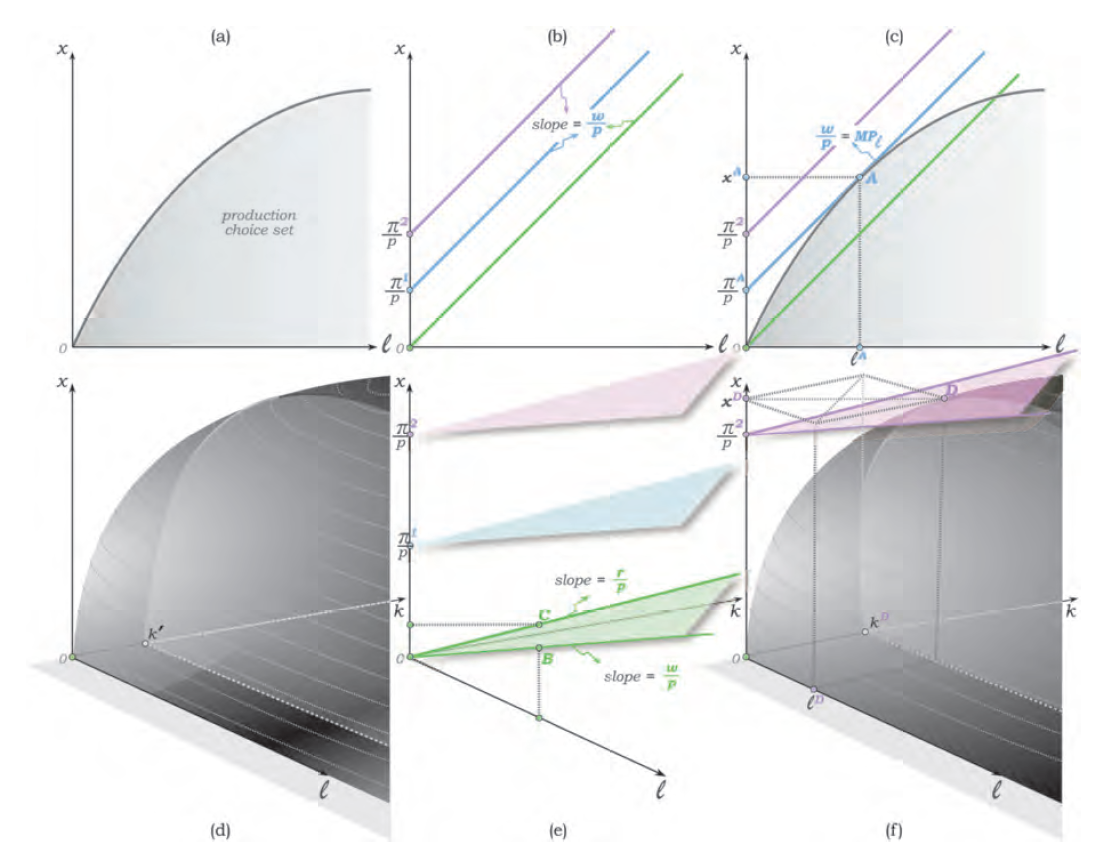
\includegraphics[width=1\textwidth]{12_1} %插入图片,[]中设置图片大小,{}中是图片文件名
	\caption{Profit Maximization in the Single-Input and Two-Input Model} %最终文档中希望显示的图片标题
	\label{Fig.main2} %用于文内引用的标签
\end{figure}

利润最大化表明:
\[
MP_l=\frac{w}{p}\enspace and\enspace MP_k=\frac{r}{p}
\]
\[
MRP_l=pMP_l=w\enspace and\enspace MRP_k=pMP_k=r
\]

\subsection{两要素生产集:等产量线与规模报酬}
等产量线是从生产边界中得到的,它表示了生产者所面临的技术限制(constraint)。而无差异曲线代表了消费者选择问题中的偏好(tastes)而非限制。

其次,在消费者理论中,效用本身无法用任何客观方法来衡量,因此无差异曲线的数值并不存在客观的解释,而仅仅代表序数关系。然而对于代表生产某一特定产量而不是幸福的要素投入集合的等产量线来说,却并不是这样。产出是一种我们可以客观度量的量,将同一张等产量线图上的等产量值重新标记会以经济上有意义的方式改变三维的生产技术。

\hspace*{\fill}

TRS和边际产出

等产量线的斜率即边际技术替代率(marginal technical rate of substitution)。
\[
TRS=\frac{MP_l}{MP_k}
\]

\hspace*{\fill}

等产量线和消费者无差异曲线在技术上的相似性:

(1)越多越好(单调性);

(2)平均优于极端(凸性);

(3)当在生产中投入增加了一个极少的量时,“在生产中无突然的暴涨”(连续性)。

第二,等产量线上的TRS改变率表明了生产过程中不同投入的替代程度,正如无差异曲线上MRS的改变率表明了消费者对不同商品偏好的替代程度。

\hspace*{\fill}

规模报酬和生产选择集的凸性

在无差异曲线或等产量线上方的要素投入集合,有时被称为“上水平集”,我们所使用的“凸性”源于上水平集为凸的事实,即“平均优于极端”。

一个(三维)生产集的凸性不同于对生产集进行横切所产生的上水平集的凸性。

如果一个集合是凸的,则从集合中任选两点A和B,它们的连线都在此集合中。对于三维生产选择集,若使之为凸,则它必须满足每一个水平切面所形成的集合都是凸的。但是仅仅知道“平均优于极端”不足以保证我们的三维的生产选择集本身是凸的,因为“平均优于极端”仅仅意味着生产选择集的水平切面是凸的,整个生产选择集不都是凸的,除非它的纵向切面也都是凸的。

\begin{figure}[H] %H为当前位置,!htb为忽略美学标准,htbp为浮动图形
	\centering %图片居中
	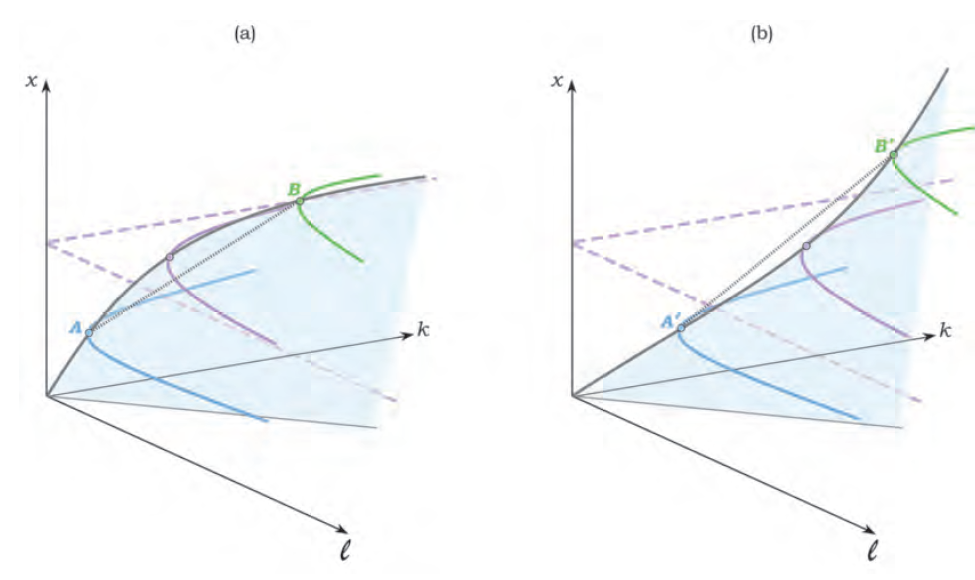
\includegraphics[width=1\textwidth]{12_2} %插入图片,[]中设置图片大小,{}中是图片文件名
	\caption{Convex and Non-Convex Producer Choice Sets} %最终文档中希望显示的图片标题
	\label{Fig.main3} %用于文内引用的标签
\end{figure}

\begin{figure}[H] %H为当前位置,!htb为忽略美学标准,htbp为浮动图形
	\centering %图片居中
	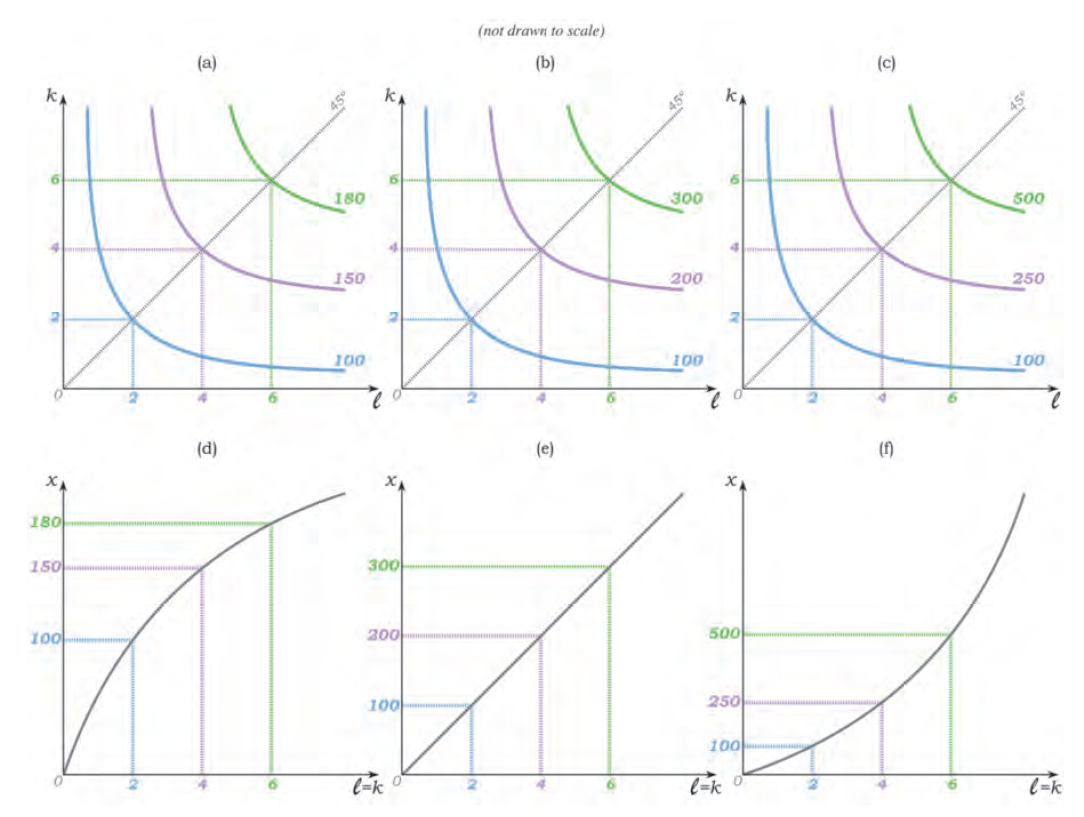
\includegraphics[width=1\textwidth]{12_3} %插入图片,[]中设置图片大小,{}中是图片文件名
	\caption{Homothetic Isoquant Maps Can Represent Increasing, Constant, or Decreasing Returns to Scale
		Production Processes} %最终文档中希望显示的图片标题
	\label{Fig.main4} %用于文内引用的标签
\end{figure}

若上图中的x都代表效用,则两幅图的含义完全一致,因为图(b)仅是对效用轴的按大小进行了变换,而无差异曲线的形状没有发生变化。

规模报酬递减:投入增加t倍,产出增加小于t倍;

规模报酬不变:投入增加t倍,产出增加等于t倍;

规模报酬递增:投入增加t倍,产出增加大于t倍。

\hspace*{\fill}

规模报酬与边际产出递减

一种投入的边际产出被定义为在其他投入不变的情况下,增加一单位的该投入所引起的产出的增加。如果说所有边际产出是递减的,则意味着当我们控制某种投入之外其他所有投入不变时,增加额外单位的该投入所引起的产出增加会比之前引起的增加要少。

\hspace*{\fill}

在位似生产函数的情形下:

规模报酬递减可以推出所有要素边际产出递减;

一种要素边际产出递增可以推出规模报酬递增。

\subsection{在利润最大化的过程中成本最小化}

技术有效:在生产边界上生产(没有资源浪费);

经济有效:最便宜。

由于在成本最小化的要素投入组合上时,等产量线的斜率一定等于等成本线的斜率,因此成本最小化意味着:
\[
TRS=\frac{MP_l}{MP_k}=\frac{w}{r}
\]

根据成本曲线来最大化利润:

在单一要素投入模型中推导利润最大化的逻辑在两种要素投入时也成立——此时价格等于MC。

成本曲线上的每一个点都是生产者在生产某个产出水平时最小化成本得到的。

还有一种理论上可行的解:生产者的最优选择可能是生产一个无穷大的产量——规模报酬递增时出现。

\subsection{把成本最小化和利润最大化结合起来}

一个仅仅将成本最小化的生产者不会注意产出的价格;ta所需要决定的是,对于给定的投入价格(w,r),找到在生产不同产出量时成本最小(经济有效)的方法。
\[
TRS=\frac{MP_l}{MP_k}=\frac{w}{r}
\]

而一个利润最大化的生产者还会考虑产出价格,并且会在每个要素的边际收益产品等于要素价格的时候进行生产。
\[
MRP_l=pMP_l=w\enspace and\enspace MRP_k=pMP_k=r
\]

因此利润最大化的生产者实质上已经进行了成本最小化,但反过来就不一定成立。只有当成本最小化的生产者依据$ p=MC $(只要MC大于AC)来确定产出水平时,他们才能成为利润最大化的生产者,这与说利润最大化的生产者在边际收益产品等于要素价格处进行生产是一样的。

\section{多要素模型背后的数学分析}
\subsection{生产者选择集和生产函数}
生产者选择集被定义为技术可行的生产计划集$ (x,l,k) $:
\[
C(f:\mathbb{R}^2_+\rightarrow\mathbb{R}^1_+)=\{(x,l,k)\in\mathbb{R}^3|x\le f(l,k)\}
\]

边际产出与TRS:
\[
MP_l=\frac{\partial f(l,k)}{\partial l}\enspace and\enspace MP_k=\frac{\partial f(l,k)}{\partial k}
\]
\[
TRS=\frac{\partial f(l,k)/\partial l}{\partial f(l,k)/\partial k}
\]

\hspace*{\fill}

“平均优于极端”与拟凹性:“平均优于极端”是指在同一等产量线上的两个要素组合的均值组合至少会生产出至少和这个两个极值组合一样多(一般更多)的产出。

考虑一个函数$ f:\mathbb{R}^2_+\rightarrow \mathbb{R}^1 $,其是拟凹的(quasiconcave),当且仅当对于任意的在$ \mathbb{R}^2_+ $中的两点$ A=(x^A_1,x^A_2) $和$ B=(x^B_1,x^B_2) $以及任意$ \alpha\in(0,1) $

\[
min\{f(x^A_1,x^A_2),f(x^B_1,x^B_2)\}\le f(\alpha x^A_1+(1-\alpha)x^B_1),\alpha x^A_2+(1-\alpha)x^B_2)
\]

考虑在同一等产量线上的两个要素组合$ A=(l^A,k^A) $和$ B=(l^B,k^B) $,由于在同一条等产量线上,因此$ f(l^A,k^A)=f(l^B,k^B) $,通过对于拟凹性的定义,可以推断要素组合的任意加权平均至少等于A和B所在的等产量线所代表的产量。因此拟凹的生产函数代表了要素组合的均值的产量高于要素组合的极值的产量的生产过程。

拟凹的生产函数的等产量线有凸的上水平集,并且等产量线有凸的上水平集的生产过程一定具有拟凹的生产函数。所有满足“平均优于极端”的效用函数都是拟凹的。

\hspace*{\fill}

函数$ f:\mathbb{R}^2_+\rightarrow\mathbb{R}^1 $是凹的,当且仅当对于$ \mathbb{R}^2_+ $中的任意两点$ A=(x^A_1,x^A_2) $和$ B=(x^B_1,x^B_2) $以及任意$ \alpha\in(0,1) $,
\[
\alpha f(x^A_1,x^A_2)+(1-\alpha)f(x^B_1,x^B_2)\le f(\alpha x^A_1+(1-\alpha)x^B_1),\alpha x^A_2+(1-\alpha)x^B_2)
\]

很容易看出,每一个凹函数都是拟凹的,因为对于任意两点$ A=(x^A_1,x^A_2) $和$ B=(x^B_1,x^B_2) $,以及任意$ \alpha\in (0,1) $在满足拟凹时下面不等式总是成立的:
\[
min\{f(x^A_1,x^A_2),f(x^B_1,x^B_2)\}\le \alpha f(x^A_1,x^A_2)+(1-\alpha)f(x^B_1,x^B_2)
\]
然而反过来不成立。 

\begin{figure}[H] %H为当前位置,!htb为忽略美学标准,htbp为浮动图形
	\centering %图片居中
	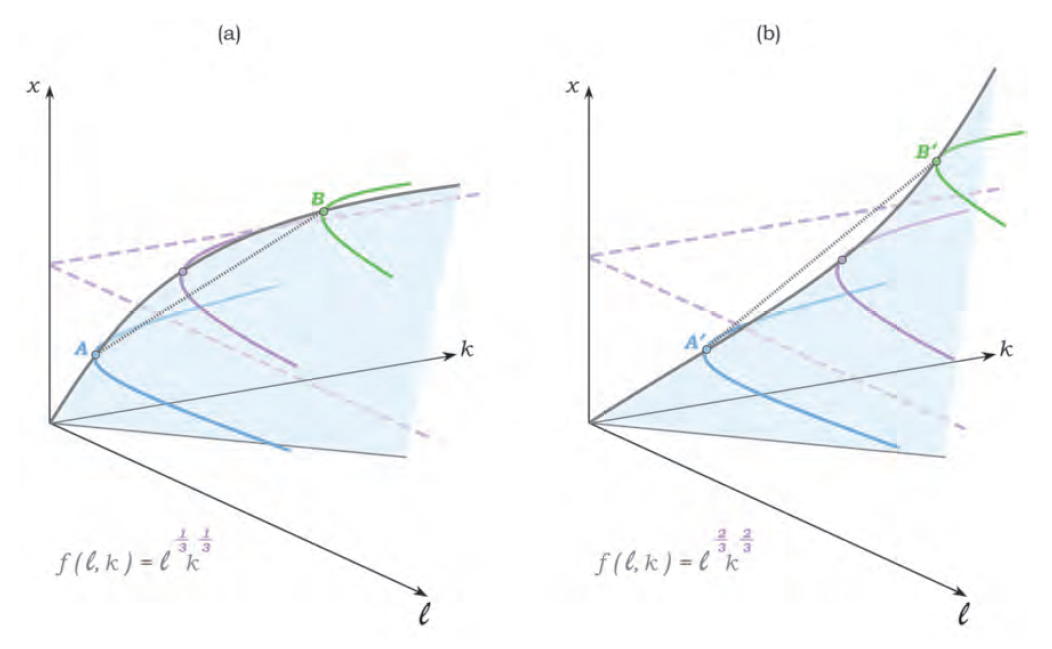
\includegraphics[width=1\textwidth]{12_4} %插入图片,[]中设置图片大小,{}中是图片文件名
	\caption{Quasiconcave Functions Can Be Concave (a) but Don’t Have to Be (b)} %最终文档中希望显示的图片标题
	\label{Fig.main5} %用于文内引用的标签
\end{figure}

\hspace*{\fill}

规模报酬和凹性

当等产量线的图是位似的时,凸生产选择集的边界可由一个规模报酬递减的凹函数来表示。而边际报酬递增表明生产选择集的非凹性和生产函数的非凹性。

齐次函数都是位似的,一个函数是k阶齐次的,当且仅当
\[
f(tl,tk)=t^kf(l,k)
\]

规模报酬不变的生产函数是一阶齐次的,规模报酬递减的生产函数是齐次的并且齐次的阶数小于1,规模报酬递增的生产函数是齐次的并且齐次的阶数大于1。不是所有的位似函数都是齐次的。

\hspace*{\fill}

规模报酬与边际产品递减
\[
MP_l=\alpha l^{\alpha-1}k^\beta\enspace and MP_k=\beta l^\alpha k^(\beta-1)
\]

这个生产函数具有递减的MP,当且仅当MP的导数为负时:
\[
\frac{\partial MP_l}{\partial l}=\alpha(\alpha-1)l^{\alpha-2}k^\beta\enspace and \enspace\frac{\partial MP_k}{\partial k}=\beta(\beta-1)l^\alpha k^{\beta-2}
\]

因此仅当每个指数都小于1的时候,劳动和资本的边际产出才是递减的。

\subsection{等利润平面与利润最大化}

生产计划$ (x,l,k) $下的利润$ \pi $为
\[
\pi=px-wl-rk
\]

等利润面定义为:
\[
P(\pi,p,w,r)=\{(x,l,k)\in\mathbb{R}^3|\pi=px-wl-rk\}
\]

利润最大化问题:

\[
\max\limits_{x,l,k}=px-wl-rk\enspace s.t.\enspace x=f(l,k)
\]
从上式中得出要素需求函数
\[
l(p,w,r)\enspace and\enspace k(p,w,r)
\]
将二者代入生产函数中,得到供给函数
\[
x(p,w,r)=f(l(p,w,r),k(p,w,r))
\]

\subsection{在利润最大化的过程中成本最小化}

单一要素投入的和多要素投入模型的区别在于:单一要素投入模型的技术有效的生产计划就是默认的经济有效的生产计划。

成本最小化问题:
\[
\min\limits_{l,k}=wl+rk\enspace s.t.\enspace x=f(l,k)
\]
可以导出条件要素需求函数:
\[
l(w,r,x)\enspace and k(w,r,x)
\]

条件要素需求函数告诉我们,在生产x单位的条件下生产者在现行工资和租金水平下使用多少劳动和资本。

\hspace*{\fill}

如果知道条件要素需求函数,就可以得到任意投入要素价格在任意产出水平时的最小成本,即成本函数:
\[
C(w,r,x)=wl(w,r,x)+rk(w,r,x)
\]

从成本函数C可以导出供给函数(运用$ p=MC $)。最后,通过把这个供给函数代回到条件要素需求函数中,就可以推导出实际的要素需求函数。

\begin{figure}[H] %H为当前位置,!htb为忽略美学标准,htbp为浮动图形
	\centering %图片居中
	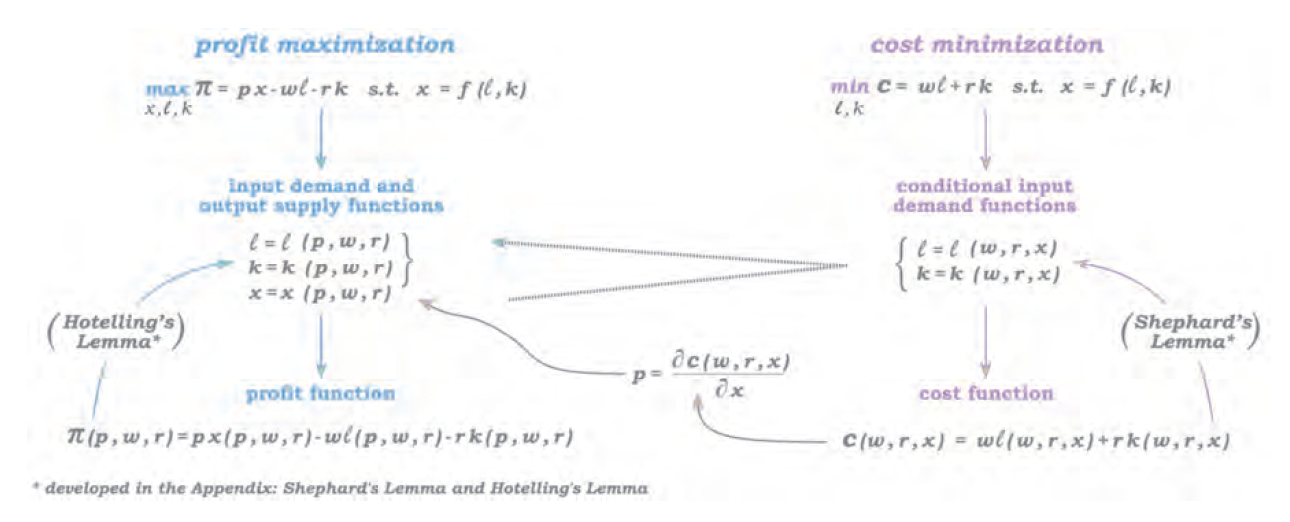
\includegraphics[width=1\textwidth]{12_5} %插入图片,[]中设置图片大小,{}中是图片文件名
	\caption{“Duality” of Profit Maximization and Cost Minimization} %最终文档中希望显示的图片标题
	\label{Fig.main6} %用于文内引用的标签
\end{figure}

\hspace*{\fill}

比较消费者理论和生产者理论:

消费者的支出最小化问题可以等同于生产者成本最小化问题。

消费者理论中的希克斯需求函数类似于生产者理论中的条件要素需求函数,前者总是假设有足够的钱达到一个效用水平,在不同的产出价格下ta将要购买的消费组合,后者告诉我们假设生产者总是有足够的钱来达到一条给定的产出水平,在不同的要素投入价格下ta将会购买的要素投入组合。

消费者理论的支出函数类似于生产者理论的成本函数,前者告诉我们对于要达到效用水平u的消费者在不同的产出价格下所需的最小支出,而后者告诉我们对于要达到产量水平x的生产者在不同的要素投入价格下所需的最小成本。

生产者理论的对偶图的左侧与消费者理论不同:消费者理论中效用函数是效用最大化中的目标方程,生产者理论中的生产函数是利润最大化中的限制条件。

消费者理论对偶图的右侧只反映替代效应,生产者理论中也有类似的条件要素需求的替代效应。消费者理论对偶图左侧的收入效应使消费者理论变得复杂,这种情况的出现是因为效用函数的最大化是在预算约束下进行的。而生产者则没有预算限制;如果他们能够通过生产来获得利润,那么收益可以支付成本。

\section{Appendix 支出函数和利润函数的性质}
Shephard's Lemma:
\[
\frac{\partial C(w,r,x)}{\partial w}=l(w,r,x)\enspace \frac{\partial C(w,r,x)}{\partial r}=k(w,r,x)
\]
条件要素需求函数总是向下倾斜的:
\[
\frac{\partial l(w,r,x)}{\partial w}\le0\enspace \frac{\partial k(w,r,x)}{\partial r}\le0
\]

Hotelling's Lemma
\[
\frac{\partial \pi(p,w,r)}{\partial p}=x(p,w,r)
\]
\[
\frac{\partial \pi(p,w,r)}{\partial w}=-l(p,w,r)
\]
\[
\frac{\partial \pi(p,w,r)}{\partial k}=-k(p,w,r)
\]

利润函数$ \pi(p,w^A) $是关于产出价格的凸函数,而且这个函数在$ p^A $的斜率为$ x^A=x(p^A,w^A) $,即:
\[
\frac{\partial \pi(p^A,w^A)}{\partial p}=x(p^A,w^A)
\]

利润函数关于投入要素是凸函数而且这个函数在$ p^A $的斜率为$ x^A=-l(p^A,w^A) $,即:
\[
\frac{\partial \pi(p^A,w^A)}{\partial w}=-l(p^A,w^A)
\]


\end{document}